\chapter{Continuous Random Variables and Probability Distribution}

\section{Probability Density Functions and Cumulative Distribution Functions}

\subsection{Probability Distributions for Continuous Variables}

\begin{definition}
    Let $X$ be a continuous rv. Then a \textbf{probability distribution} or \textbf{probability density function}(pdf) of $X$ is a function $f(x)$ such that for any two numbers $a$ and $b$ with $a\leq b$,

    \begin{align*}
        P(a\leq X\leq b) = \int_a^bf(x)dx
    \end{align*}

    That is, the probability that $X$ takes on a value in the interval[a, b] is the area above this interval and under the graph of the density function. The graph of $f(x)$ is often referred to as the \textit{density curve}.

    A legitimate pdf $f(x)$ must satisfy the following two conditions:

    \begin{enumerate}
        \item $f(x)\geq 0$ for all $x$
        \item $\int_{-\infty}^\infty f(x)dx = [{\rm area\ under\ the\ entire\ graph\ of\ }f(x)] = 1$
    \end{enumerate}
\end{definition}

\begin{definition}
    A continuous rv $X$ is said to have a \textbf{uniform distribution} on the interval $[A, B]$ if the pdf of $X$ is 

    \begin{align*}
        f(x;A,B) = \left\{\begin{array}{cl}
            \frac{1}{B-A} & A\leq X\leq B \\
            0 & {\rm otherwise} \\
        \end{array}\right. \\
    \end{align*}
\end{definition}

\subsection{The Cumulative Distribution Function}

\begin{definition}
    The \textbf{cumulative distribution function} $F(x)$ for a continuous rv $X$ is defined for every number $x$ by

    \begin{align*}
        F(x) = P(X\leq x) = \int_{-\infty}^\infty f(y)dy
    \end{align*}
    For each $x$, $F(x)$ is the area under the density curve to the left of $x$.
\end{definition}

\subsection{Using $F(x)$ to Compute Probabilities}

\begin{proposition}
    Let $X$ be a continuous rv with pdf $f(x)$ and cdf $F(x)$. Then for any number $a$,

    \begin{align*}
        P(X>a) = 1-F(a) \\
    \end{align*}

    and for any two numbers $a$ and $b$ with $a<b$,

    \begin{align*}
        P(a\leq X\leq b) = F(b) - F(a)
    \end{align*}
\end{proposition}

\subsection{Obtaining $f(x)$ from $F(x)$}

\begin{proposition}
    If $X$ is a continuous rv with pdf $f(x)$ and cdf $F(x)$, then at every $x$ at which the derivative $F'(x)$ exists, $F'(x) = f(x)$.
\end{proposition}

\subsection{Percentiles of a Continuous Distribution}

\begin{definition}
    Let $p$ be a number between 0 and 1, The (100$p$)th percentile of the distribution of a continuous rv $X$, denoted by $\eta(p)$, is defiend by

    \begin{align*}
        p = F[\eta(p)] = \int_{-\infty}^{\eta(p)} f(y) dy \\
    \end{align*}
\end{definition}

\begin{definition}
    The \textbf{median} of a continuous distribution, denoted by $\tilde{\mu}$, is the 50th percentile, so $\tilde{\mu}$ satisfies $.5=F(\tilde{\mu})$. That is, half the area under the density curve is to the left of $\tilde{\mu}$ and half os tp the right of $\tilde{\mu}$.
\end{definition}

\section{Expected Values and Moment Generating Functions}

\subsection{Expected Values}

\begin{definition}
    The \textbf{expected} or \textbf{mean value} of a continuous rv $X$ with pdf $f(x)$ is

    \begin{align*}
        \mu_X = E(X) = \int_{-\infty}^\infty x\cdot f(x)dx \\
    \end{align*}

    This expected value will exist provided that $\int_{-\infty}^\infty |x|f(x)dx < \infty$.
\end{definition}

\begin{proposition}
    If $X$ is a continuous rv with pdf $f(x)$ and $h(X)$ is any function of $X$, then

    \begin{align*}
        E[h(X)] = \mu_{h(X)} = \int_{-\infty}^\infty h(x)\cdot f(x) dx \\
    \end{align*}

    This expected value will exist provided that $\int_{-\infty}^\infty |h(x)|f(x) dx < \infty$.
\end{proposition}

\subsection{The Variance and Standard Deviation}

\begin{definition}
    The \textbf{variance} of a continuous random variable $X$ with pdf $f(x)$ and mean value $\mu$ is

    \begin{align*}
        \sigma_X^2 = V(X) = \int_{-\infty}^\infty (x-\mu)^2\cdot f(x) dx = E[(X-\mu)^2] \\
    \end{align*}

    The \textbf{standard deviation}(SD) of $X$ is $\sigma_X = \sqrt{V(X)}$.

    Also,

    \begin{align*}
        V(X) = E(X^2) - [E(X)]^2 \\
    \end{align*}
\end{definition}

\subsection{Approximating the Mean Value and Standard Deviation}

\begin{proposition}
    Suppose $h(x)$ is differentiable and that its derivative evaluated at $\mu$ satisfies $h'(\mu)\neq 0$. Then if the variance of $X$ is small, which means the distribution of $X$ is largely concentrated on an interval of values close to $\mu$, the mean value and variance of $Y=h(X)$ can be approximated as follows:

    \begin{align*}
        E[h(X)] \approx h(\mu),\quad V[h(X)] \approx [h'(\mu)]^2\sigma^2 \\
    \end{align*}
\end{proposition}

\subsection{Moment Generating Functions}

\begin{definition}
    The \textbf{moment generating function}(mgf) of a continuous random variable $X$ is 

    \begin{align*}
        M_X(t) = E(e^{tX}) = \int_{-\infty}^\infty e^{tX} f(x) dx. \\
    \end{align*}

    As in the discrete case, we will say that the moment generating function exists if $M_X(t)$ is defined for an interval of numbers that includes zero in tis interior, which mean that it includes both positive and negative values ot $t$.

    Just as before, when $t=0$ the value of the mgf is always 1:

    \begin{align*}
        M_X(0) = E(e^{0X}) = \int_{-\infty}^\infty e^{0x} f(x) dx = \int_{-\infty}^\infty f(x) dx = 1 \\
    \end{align*}
\end{definition}

\begin{proposition}
    Two continuous distributions have the same pdf if and only if they have the same moment generating function, assuming that the mgf exists.
\end{proposition}

\begin{proposition}
    For continuous rv $X$, if mgf exists, 

    \begin{align*}
        E(X^r) = M_X^{(r)}(0) \\
    \end{align*}

    A faster version of deriving mean and variance of $X$ if mgf exists is

    \begin{align*}
        \mu & = E(X) = R_X'(0) \\
        \sigma^2 & = V(X) =R_X '' (0) \\
    \end{align*}

    where $R_X(t) = \ln[M_X(t)]$.
\end{proposition}

\begin{proposition}
    For continuous rv $X$ and linear function $Y=aX+b$, if mgf $M_X(t)$ exists, then 

    \begin{align*}
        M_Y(t) = e^{bt}M_X(at) \\
    \end{align*}
\end{proposition}

\section{The Normal Distribution}

\begin{definition}
    A continuous rv $X$ is said to have a \textbf{normal distribution} with parameters $\mu$ and $\sigma$(or $\mu$ and $\sigma^2$), where $-\infty < \mu < \infty$ and $0 < \sigma$, if the pdf of $X$ is 

    \begin{align*}
        f(x;\mu,\sigma) = \frac{1}{\sqrt{2\pi}\sigma} e^{-(x-\mu)^2/(2\sigma^2)} \quad -\infty<x<\infty \\
    \end{align*}
\end{definition}

\subsection{The Standard Normal Distribution}

\begin{definition}
    The normal distribution with parameter values $\mu = 0$ and $\sigma = 1$ is called the \textbf{standard normal distribution}. A random variable that has a standard normal distribution is called a \textbf{standard normal random variable} and will be denoted by $Z$. The pdf of $Z$ is 

    \begin{align*}
        f(z;0,1) = \frac{1}{\sqrt{2\pi}}e^{-z^2/2}\quad -\infty<z<\infty \\
    \end{align*}

    The cdf of $Z$ is $P(Z\leq z) = \int_{-\infty}^z f(y,0,1) dy$, which we will denote by $\Phi(z)$.
\end{definition}

\subsection{Percentiles of the Standard Normal Distribution}

\begin{notation}
    $z_\alpha$ will denote the value on the measurement axis for which $\alpha$ of the area under the $z$ curve lies to the right of $z_\alpha$.
\end{notation}

\begin{figure}[H]
    \centering
    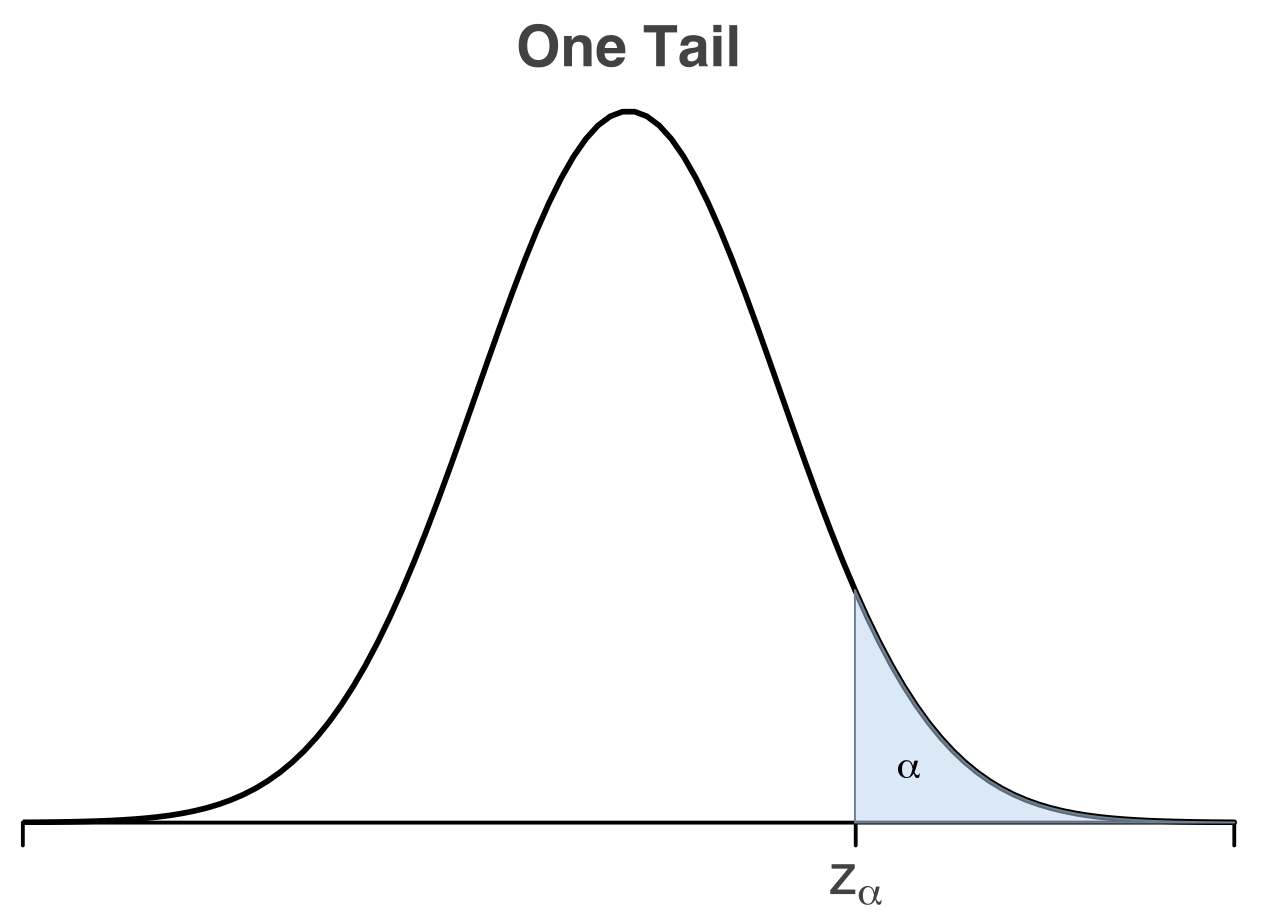
\includegraphics[width=.4\textwidth]{img/4-z-alpha-1}
    \caption{One-tail z critical value}
    \label{fig:4-1}

    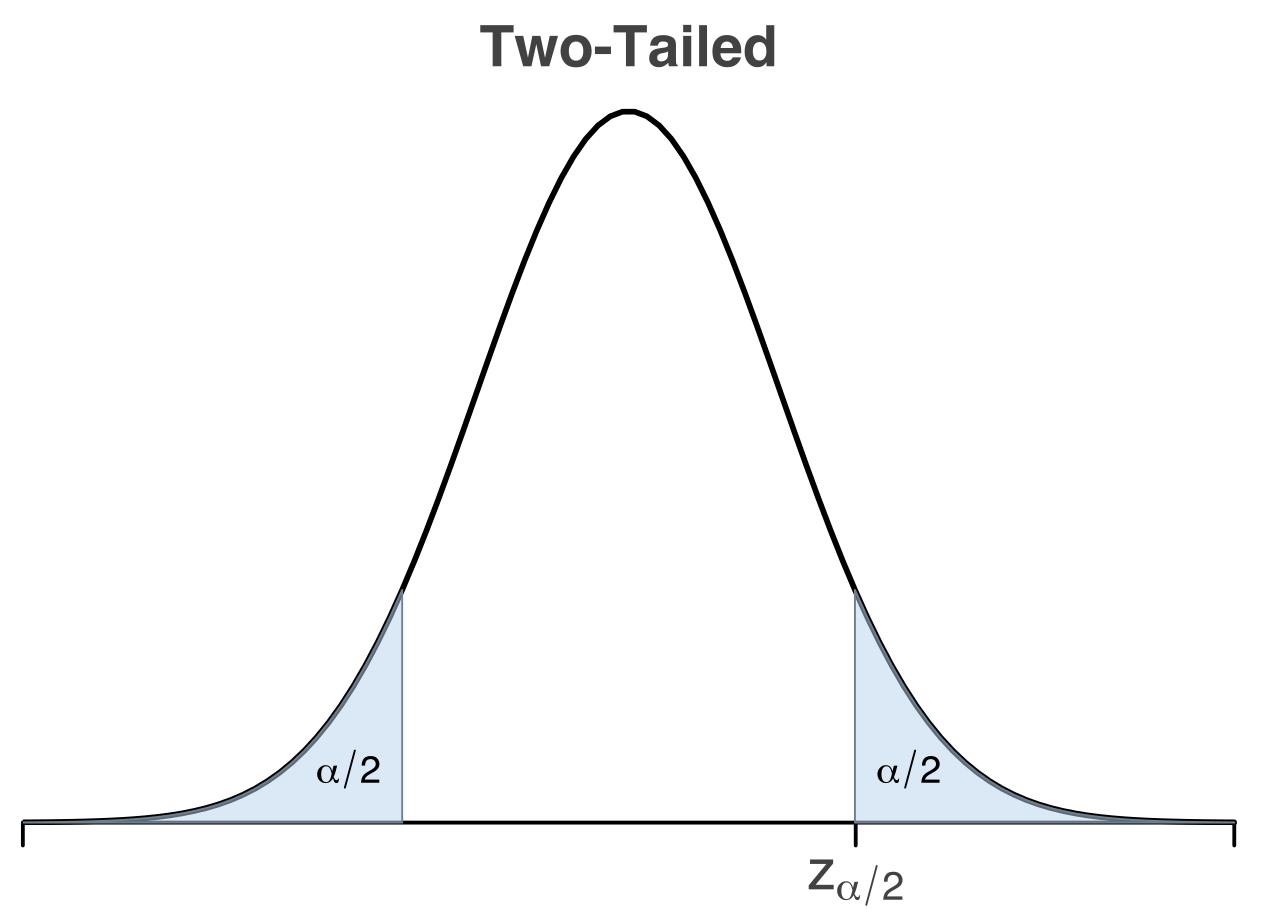
\includegraphics[width=.4\textwidth]{img/4-z-alpha-2}
    \caption{Two-tail z critical value}
    \label{fig:4-2}
\end{figure}

\subsection{Nonstandard Normal Distribution}

\begin{proposition}
    If $X$ has a normal distribution with mean $\mu$ and standard deviation $\sigma$, then

    \begin{align*}
        Z = \frac{X - \mu}{\sigma} \\
    \end{align*}

    has a standard normal distribution. Thus

    \begin{align*}
        P(a\leq X\leq b) & = P\left(\frac{a-\mu}{\sigma}\leq Z\leq \frac{b-\mu}{\sigma}\right) \\
        & = \Phi\left(\frac{b-\mu}{\sigma}\right) - \Phi\left(\frac{a-\mu}{\sigma}\right) \\
    \end{align*}

    \begin{align*}
        P(X\leq a) = \Phi\left(\frac{a-\mu}{\sigma}\right)\quad P(X\geq b) = 1-\Phi(\frac{b-\mu}{\sigma}) \\
    \end{align*}
\end{proposition}

\begin{proposition}{THE EMPIRICAL RULE}
    If the population distribution of a variable is (approximately) nomal, then

    \begin{enumerate}
        \item Roughly 68\% of the values are within 1 SD of the mean.
        \item Roughly 95\% of the values are within 2 SD of the mean.
        \item Roughly 99.7\% of the values are within 3 SD of the mean.
    \end{enumerate}
\end{proposition}

\begin{proposition}
    ~\\(100$p$)th percentile for normal($\mu,\sigma$) = $\mu + [(100p)$th percentile for standard normal]$\cdot\sigma$
\end{proposition}

\subsection{Approximating the Binomial Distribution}

\begin{proposition}
    Let $X$ be a binomial rv based on $n$ trials with success probability $p$. Then if the binomial probability histogram is not too skewed, $X$ has approximately a normal distribution with $\mu = np$ and $\sigma = \sqrt{npq}$. In particular, for $x=a$ possible value of $X$,

    \begin{align*}
        P(x\leq X) = B(x;n,p) & \approx ({\rm area\ under\ the\ normal\ curve\ to\ the\ left\ of\ }x + .5) \\
        & = \Phi\left(\frac{x+.5-np}{\sqrt{npq}}\right) \\
    \end{align*}

    In practice, the approximation in adequate provided that both $np\geq 10$ and $nq\geq 10$.
\end{proposition}

\subsection{The Normal Moment Generating Function}

\begin{proposition}
    The moment generating function of a normally distributed rv $X$ is 

    \begin{align*}
        M_X(t) = e^{\mu t + \sigma^2t^2/2} \\
    \end{align*}
\end{proposition}

\begin{proof}
    See textbook Page 191.
\end{proof}

\section{The Gamma Distribution and Its Relatives}

\begin{definition}
    For $\alpha > 0$, the \textbf{gamma function} $\Gamma(\alpha)$ is defined by

    \begin{align*}
        \Gamma(\alpha) = \int_0^\infty x^{\alpha-1}e^{-x}dx \\
    \end{align*}

    Properties of the gamma function are the following:

    \begin{enumerate}
        \item For any $\alpha>0$, $\Gamma(\alpha) = (\alpha - 1)\cdot \Gamma(\alpha - 1)$(via integration by parts)
        \item For any positive integer $n$, $\Gamma(n) = (n-1)!$
        \item $\Gamma(1/2) = \sqrt{\pi}$
    \end{enumerate}
\end{definition}

\subsection{The Family of Gamma Distributions}

\begin{definition}
    A continuous rv $X$ is said to have a \textbf{gamma dsitribution} if the pdf of $X$ is 

    \begin{align*}
        f(x;\alpha,\beta) = \left\{\begin{array}{cl}
            \frac{1}{\beta^\alpha\Gamma(\alpha)}x^{\alpha-1}e^{-x/\beta} & x>0 \\
            0 & {\rm otherwise} \\
        \end{array}\right.
    \end{align*}

    where the paramters $\alpha$ and $\beta$ satisfy $\alpha>0$, $\beta>0$. The \textbf{standard gamma distribution} has $\beta=1$, so the pdf of a standard gamma rv is 

    \begin{align*}
        f(x;\alpha,\beta) = \left\{\begin{array}{cl}
            \frac{x^{\alpha-1}e^{-x/\beta}}{\beta^\alpha\Gamma(\alpha)} & x>0 \\
            0 & {\rm otherwise} \\
        \end{array}\right.
    \end{align*}
\end{definition}

\begin{proposition}
    The moment generating function of a gamma rv is
    
    \begin{align*}
        M_X(t) = \frac{1}{(1-\beta t)^\alpha} \\
    \end{align*}
\end{proposition}

\begin{proof}
    See textbook Page 196.
\end{proof}

\begin{proposition}
    The mean and variance of a rv $X$ having the gamma distribution $f(x;\alpha,\beta)$ are
    
    \begin{align*}
        E(X) = \mu = \alpha\beta \quad V(X) = \sigma^2 = \alpha\beta^2 \\
    \end{align*}
\end{proposition}

\begin{proposition}
    cdf of standard gamma rv $X$ is

    \begin{align*}
        F(x;\alpha) = \int_0^x\frac{y^{\alpha-1}e^{-y}}{\Gamma(\alpha)} dy \quad x>0 \\
    \end{align*}

    which is also denoted as \textbf{incomplete gamma function}.
\end{proposition}

\begin{proposition}
    Let $X$ have a gamma distribution with parameters $\alpha$ and $\beta$. Then for any $x>0$, the cdf of $X$ is given by

    \begin{align*}
        F(X\leq x) = F(x;\alpha,\beta) = F(\frac{x}{\beta};\alpha) \\
    \end{align*}

    the incomplete gamma function evaluated at $x/\beta$.
\end{proposition}

\subsection{The Exponential Distribution}

\begin{definition}
    $X$ is said to have an \textbf{exponential distribution} with parameter $\lambda$($\lambda > 0$) if the pdf of $X$ is

    \begin{align*}
        f(x;\lambda) = \left\{\begin{array}{cl}
            \lambda e^{-\lambda x} & x\geq 0 \\
            0 & {\rm otherwise} \\
        \end{array}\right.
    \end{align*}
\end{definition}

\begin{proposition}
    The mean and variance of an exponential rv $X$ are

    \begin{align*}
        \mu = \alpha\beta = \frac{1}{\lambda}\quad \sigma^2 = \alpha\beta^2=\frac{1}{\lambda^2} \\
    \end{align*}

    The cdf of exponential rv $X$ is 

    \begin{align*}
        F(x;\lambda) = \left\{\begin{array}{cl}
            0 & x<0 \\
            1 - e^{-\lambda x} & x\geq 0 \\
        \end{array}\right.
    \end{align*}
\end{proposition}

\begin{proposition}
    Suppose that the number of events occurring in any time interval of length $t$ has a Poisson distribution with parameter $\alpha t$(where $\alpha$, the rate of the event process, is the expected number of events occurring in 1 unit of time) and that nubers of occurrences in nonoverlapping intervals are independent of one another. Then the distribution of elapsed tiem between the occurrence of two successive events is exponential with parameter $\lambda = \alpha$.
\end{proposition}

\begin{proposition}{MEMORYLESS PROPERTY}
    The distribution of additional lifetime is exactly the same as the original distribution of lifetime, so at each point in time the component shows no effect of wear. In other words, the distribution of remaining lifetime is independent of current age.
\end{proposition}{MEMORYLESS PROPERTY}


\subsection{The Chi-Squared Distribution}

\begin{definition}
    Let $\upsilon$ be a positive integer. Then a rv $X$ is said to have a \textbf{chi-squared distribution} with parameter $\upsilon$ if the pdf of $X$ is the gamma density with $\alpha = \upsilon / 2$ and $\beta = 2$. The pdf of a chi-squared rv is thus

    \begin{align*}
        f(x;\upsilon) = \left\{\begin{array}{cl}
            \frac{1}{2^{\upsilon/2}\Gamma(\upsilon/2)}x^{(\upsilon / 2)-1} e^{-x/2} & x\geq 0 \\
            0 & x < 0 \\
        \end{array}\right.
    \end{align*}

    The parameter $\upsilon$ is called the \textbf{number of degrees of freedom}(df) of $X$. The symbol $\chi^2$ is often used in place of "chi-squared".
\end{definition}

\section{Other Continuous Distributions}

\subsection{The Weibull Distribution}

\begin{definition}
    A rv $X$ is said to have a \textbf{Weibull distribution} with parameters $\alpha$ and $\beta$($\alpha>0$, $\beta>0$) if the pdf of $X$ is 

    \begin{align*}
        f(x;\alpha,\beta) = \left\{\begin{array}{cl}
            \frac{\alpha}{\beta^\alpha} x^{\alpha - 1} e^{-(x/\beta)^\alpha} & x\geq 0 \\
            0 & x < 0 \\
        \end{array}\right.
    \end{align*}

    The mean and variance of Weibull rv $X$ is

    \begin{align*}
        \mu = \beta\Gamma\left(1 + \frac{1}{\alpha}\right)\quad \sigma^2 = \beta^2\left\{\Gamma\left(1 + \frac{2}{\alpha}\right) - \left[\Gamma\left(1 + \frac{1}{\alpha}\right)\right]^2\right\} \\
    \end{align*}

    The cdf of a Weibull rv having parameters $\alpha$ and $\beta$ is

    \begin{align*}
        F(x;\alpha,\beta) = \left\{\begin{array}{cl}
            0 & x < 0\\
            1 - e^{-(x/\beta) ^ \alpha} & x\geq 0\\
        \end{array}\right.
    \end{align*}

    Frequently, in practical situation, a Weibull model may be reasonable except that the smallest possible $X$ may be some value $\gamma$ not assumed o be zero(this would also apply to a gamma model). The quantity $\gamma$ can then be regareded as a third parameter of the distribution. This is equivalent to saying that $X-\gamma$ has the pdf, so that the cdf of $X$ is obtained by replacing $x$ by $x-\gamma$.
\end{definition}

\subsection{The Lognormal Distribution}

\begin{definition}
    A nonnegative rv $X$ is said to have a \textbf{lognormal distribution} if the rv $Y=\ln (X)$ has a normal distribution. The resulting pdf of a lognormal rv when $\ln (X)$ is normally distributed with paramters $\mu$ and $\sigma$ is 
    
    \begin{align*}
        f(x;\mu,\sigma) = \left\{\begin{array}{cl}
            \frac{1}{\sqrt{2\pi}\sigma x} e^{-[\ln(x) - \mu]^2/(2\sigma^2)} & x\geq 0\\
            0 & x<0\\
        \end{array}\right.
    \end{align*}
    
    The $\mu$ and $\sigma$ denoted the mean and variance of $\ln(X)$.
    
    The mean and variance of $X$ can be obtained by
    
    \begin{align*}
        E(X) = e^{\mu + \sigma^2/2}\quad V(X) = e^{2\mu + \sigma^2}\cdot (e^{\sigma^2} - 1) \\
    \end{align*}

    When we only have mean and variance of lognormal rv $\ln(X)$ and value table of normal rv $X$, we obtain the cdf by

    \begin{align*}
        F(x;\mu,\sigma) & = P(X\leq x) = P[\ln (X)\leq \ln (x)] = P\left[\frac{\ln(X)-\mu}{\sigma}\leq\frac{\ln(x)-\mu}{\sigma}\right] \\
        & = P\left[Z\leq \frac{\ln(x)-\mu}{\sigma}\right] = \Phi\left[\frac{\ln(x)-\mu}{\sigma}\right] \\
    \end{align*}
\end{definition}

\subsection{The Beta Distribution}

\begin{definition}
    A rv $X$ is said to have a \textbf{beta distribution} with parameters $\alpha$, $\beta$(both positive), $A$ and $B$ if the pdf of $X$ is 

    \begin{align*}
        f(x;\alpha,\beta,A,B) = \left\{\begin{array}{cl}
            \frac{1}{B-A}\cdot\frac{\Gamma(\alpha+\beta)}{\Gamma(\alpha)\cdot\Gamma(\beta)}\left(\frac{x-A}{B-A}\right)^{\alpha-1}\left(\frac{B-x}{B-A}\right)^{\beta-1} & A\leq x\leq B \\
            0 & {\rm otherwise} \\
        \end{array}\right.
    \end{align*}

    The case $A=0$, $B=1$ gives the \textbf{standard beta distribution}.

    The mean and variance of beta rv $X$ are 

    \begin{align*}
        \mu = A + (B -A) \cdot \frac{\alpha}{\alpha + \beta} \quad \sigma^2 = \frac{(B-A)^2\alpha\beta}{(\alpha + \beta)^2(\alpha + \beta + 1)} \\
    \end{align*}

    In practice, the parameters $A$ and $B$ often denote the lower and upper bound of $X$, whereas the cdf has a potential maximum bound of $A\leq X\leq B$. See Example 4.23 in textbook Page 207.
\end{definition}

\section{Probability Plots}

\begin{definition}
    The \textbf{probability plot} is used to check a distributional assumption.
\end{definition}

\subsection{A Probability Plot}

\begin{definition}
    A plot of the $n$ pairs 

    \begin{center}
        ($[100(i-.5)/n]$th $z$ percentile, $i$th smallest observation)
    \end{center}

    on a two-dimensional coordinate system is called a \textbf{normal probability plot}. If the sample observations are in fact drawn from a normal distribution with mean value $\mu$ and standard deviation $\sigma$, the points should fall close to a straight lien with slope $\sigma$ and intercept $\mu$. Thus a plot for which the points fall close to some straight line suggests that the assumption of a normal population distribution is plausible.
\end{definition}

\subsection{Transformations of a Random Variable}

\begin{theorem}
    Let $X$ hae pdf $f_X(x)$ and let $Y=g(X)$, where $g$ is monotonic(either strictly increasing or strictly decreasing) so it has an inverse function $X=h(Y)$. Assume that $h$ has a derivative $h'(y)$. Then $f_Y(y) = f_X(h(y))|h'(y)|$.

    when it comes to discrete rv $X$ and $Y$, the derivative part is not necessary $f_Y(y) = f_X(h(y))$.
\end{theorem}

